% !TEX root = Master.tex


\begin{table}[H]
\centering
\begin{tabular}{lrrrr}
   \hline
A. parametric coefficients & Estimate & Std. Error & t-value & p-value \\ 
  (Intercept) & 1.4021 & 0.0349 & 40.1343 & $<$ 0.0001 \\ 
  bf & 0.5653 & 0.2047 & 2.7614 & 0.0078 \\ 
  ff & 1.3783 & 0.1911 & 7.2126 & $<$ 0.0001 \\ 
   \hline
B. smooth terms & edf & Ref.df & F-value & p-value \\ 
  s(time\_id) & 43.8428 & 51.0000 & 65.4139 & $<$ 0.0001 \\ 
  s(total\_markdown\_pct) & 7.5308 & 9.0000 & 88.2963 & $<$ 0.0001 \\ 
   \hline
\end{tabular}
\caption{ } 
\label{tab.gam}
\end{table}



 \begin{figure}[H]
\centering
\begin{subfigure}{.45\textwidth}
  \centering
  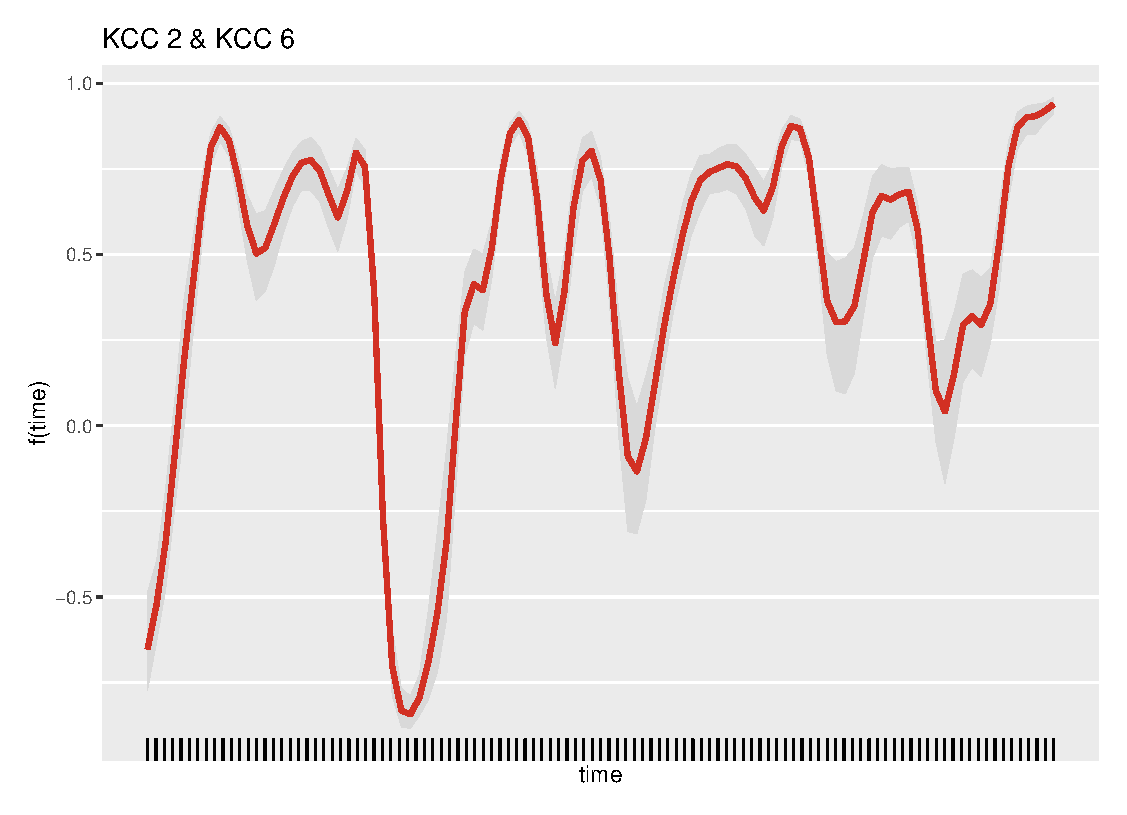
\includegraphics[width=\linewidth]{figures/time_effect_kcc_26.eps}
  \caption{Effect of time}
  \label{fig:time_effect_kcc_26}
\end{subfigure}
\begin{subfigure}{.45\textwidth}
  \centering
  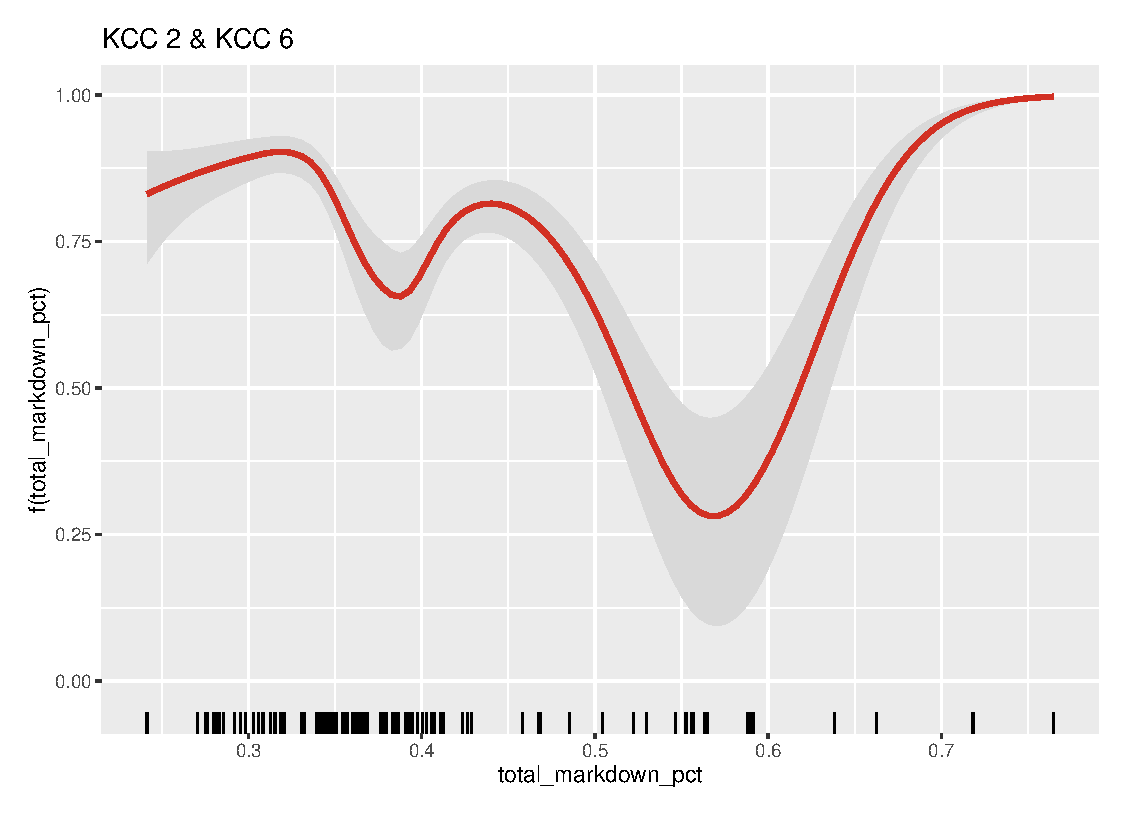
\includegraphics[width=\linewidth]{figures/markdown_effect_kcc_26.eps}
  \caption{Effect of total markdown percentage}
  \label{fig:markdown_effect_kcc_26}
\end{subfigure}
\caption{Smooth effects on Kendall's Tau: KCC 2 \& KCC 6}
\label{fig:effects_kcc_26}
\end{figure}





\begin{figure}[H]
\centering
  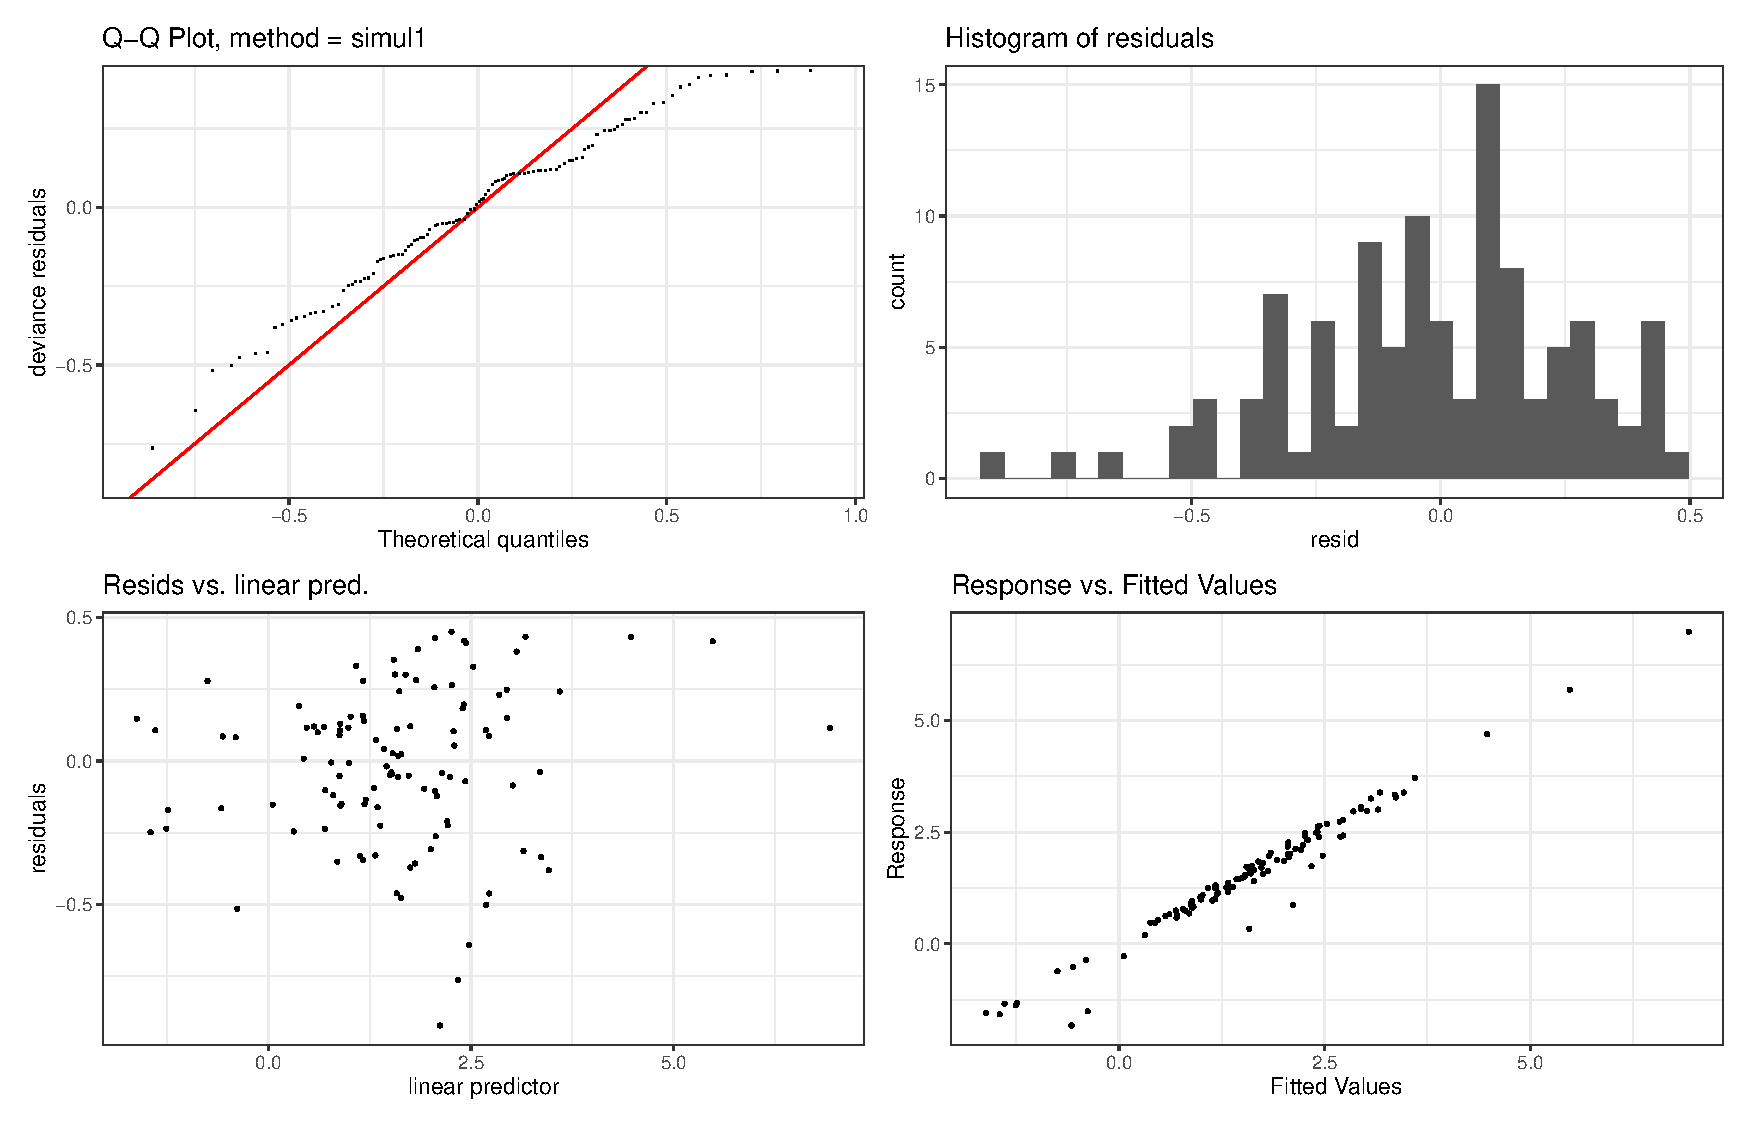
\includegraphics[width=0.9\linewidth]{figures/gam_check_kcc_26.eps}
  \caption{Check KCC 2 6}
  \label{fig:gam_check_kcc_26}
\end{figure}





 \begin{figure}[H]
\centering
\begin{subfigure}{.45\textwidth}
  \centering
  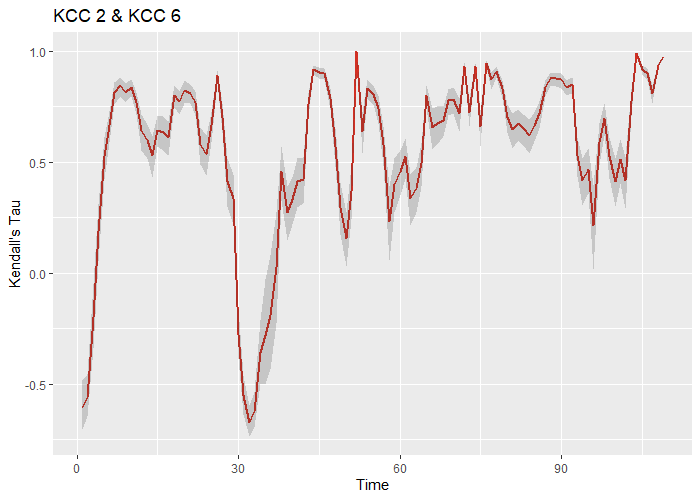
\includegraphics[width=\linewidth]{figures/tau_over_time_kcc_26.png}
  \caption{Estimates over time for KCC 2 \& KCC 6}
  \label{fig:tau_over_time_kcc_26}
\end{subfigure}
\begin{subfigure}{.45\textwidth}
  \centering
  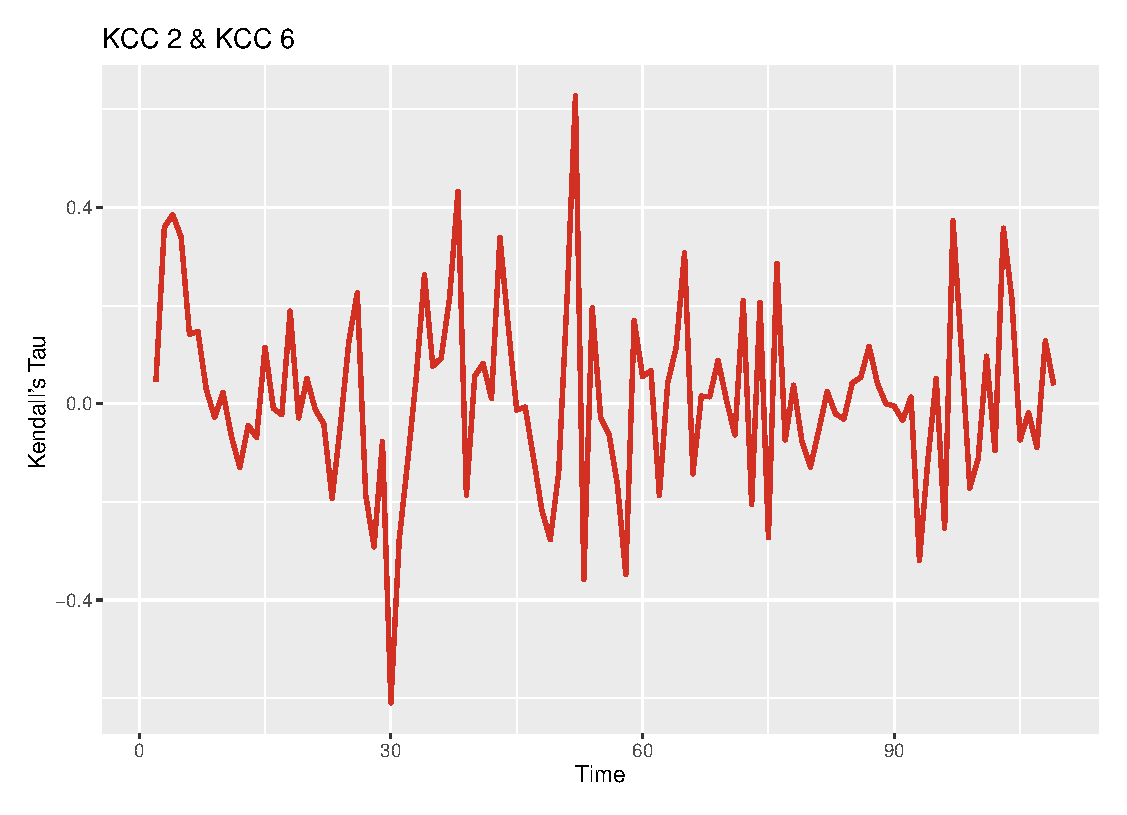
\includegraphics[width=\linewidth]{figures/diff_tau_over_time_kcc_26.eps}
  \caption{Change over time for KCC 2 \& KCC 6}
  \label{fig:diff_tau_over_time_kcc_26}
\end{subfigure}
\caption{Kendall's Tau estimates their change over time for KCC 2 \& KCC 6}
\label{fig:tau_estimates_kcc_26}
\end{figure}



